%xelatex
\documentclass[12pt]{extreport}
%\documentclass[14pt]{extreport}

\usepackage{listings}
%\usepackage{verbatim}
\usepackage{blindtext}
\usepackage[T2A]{fontenc}
\usepackage[english,ukrainian]{babel}
\usepackage{mathspec}
\setallmainfonts{Nimbus Roman}
\usepackage{graphicx}
\usepackage[a4paper,margin=0.5in]{geometry}
\usepackage{tikz}
\usetikzlibrary{calc,positioning,shapes.geometric,shapes.symbols,shapes.misc}
\usepackage{indentfirst}
\usepackage{moreverb}
\usepackage{subfiles}

\lstset{
  basicstyle=\ttfamily,
  columns=fullflexible,
  breaklines=true,
  postbreak=\raisebox{0ex}[0ex][0ex]{\color{red}$\hookrightarrow$\space}
}

\begin{document}

\subfile{title.tex}

\subsubsection*{Мета роботи}
Навчитися використовувати вказівники при написанні програм на мові С.

\subsubsection*{Завдання № 1}
З клавіатури вводиться динамічний рядок, перевірити,
чи входять у нього цифри 5 та 7. При доступі до
елементів використовувати вказівники.

\bigskip
Схема алгоритму зображена на рис. 1.

\begin{figure}[h]
	\centering
	\subfile{fch.tex}
	\caption{Схема алгоритму для першого завдання}
\end{figure}

\subsubsection*{Програмний код до першого завдання}

\begin{lstlisting}[frame=single]
#include <stdlib.h>
#include <string.h>
#include <stdio.h>

int main(){
  	char *buffer;
	int n;
	scanf("%d",&n);
	buffer = (char*)malloc((n+1) * sizeof(char));
	if(buffer == NULL) return -1;
	printf(">");
	scanf("%s",buffer);

	for(int j=0; j<n; j++){

		if(buffer[j]=='5'){
			printf("includes 5\n");
		}
		if(buffer[j]=='7'){
			printf("includes 7\n");
		}
	}

	free(buffer);
	return 0;
}
\end{lstlisting}

Вивід:
\begin{lstlisting}
527
>2175
includes 7
includes 5
\end{lstlisting}

\subsubsection*{Завдання № 2}
Задано текст. Створити масив вказівників на окремі речення. Посортувати
кожне друге речення за кодами літер. Вивести посортовані речення на екран.

\bigskip
Схема алгоритму зображена на рис. \ref{task2}

\begin{figure}[h]
	\centering
	%\subfile{fch2.tex}
	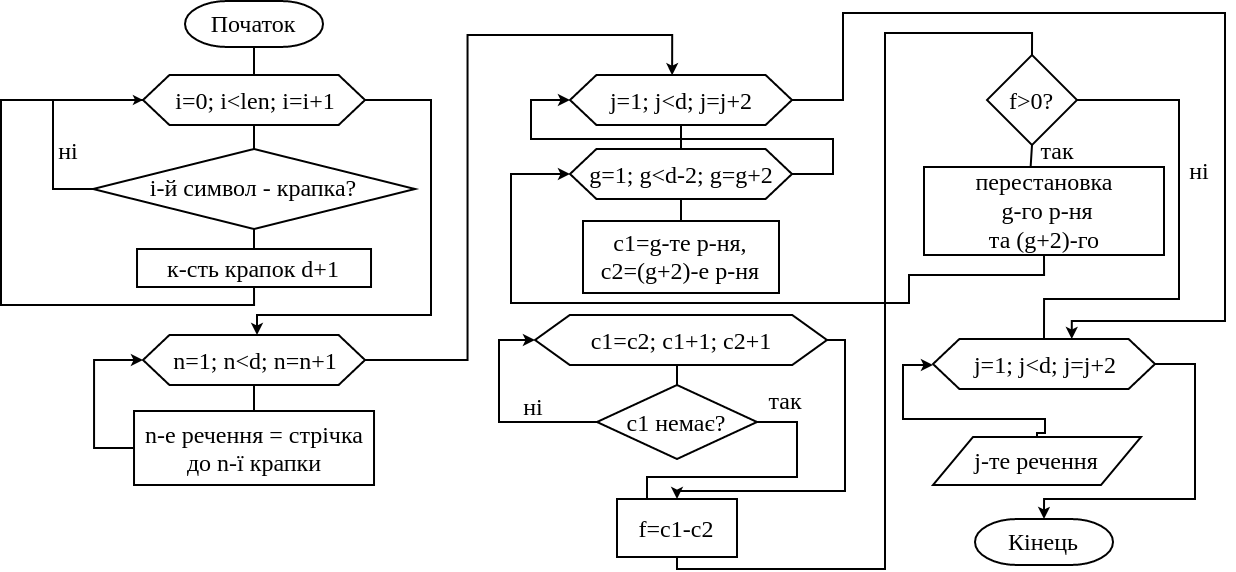
\includegraphics[width=\textwidth]{d.png}
	\caption{Схема алгоритму для другого завдання. len~--- довжина заданої стрічки}
	\label{task2}
\end{figure}

\subsubsection*{Програмний код до другого завдання}

\begin{lstlisting}[frame=single]
#include <string.h>
#include <stdio.h>

int main(){
	char arr[400]=" Lorem ipsum dolor sit amet, consectetuer adipiscing elit. Etiam lobortis facilisis sem. Nullam nec mi et neque pharetra sollicitudin. Praesent imperdiet mi nec ante. Donec ullamcorper, felis non sodales commodo, lectus velit ultrices augue, a dignissim nibh lectus placerat pede. Vivamus nunc nunc, molestie ut, ultricies vel, semper in, velit. Ut porttitor";
	int dot=0;

	for(int i=0;i<strlen(arr);i++){
	        if(arr[i] =='.')
	            dot++;
		else continue;
	        }

	char *sentence[dot+2];

	sentence[0]=strtok(arr,".");
	printf("%s\n", sentence[0]);
	for(int n=1; n<dot; n++){
		sentence[n]=strtok(NULL,".");
		printf("%s\n", sentence[n]);
	}
	/*------------------------------*/
	for(int j = 1; j < dot; j+=2){
		for(int g = 1; g < dot -2; g+=2){
			char *c1 = sentence[g];
			char *c2 = sentence[g + 2];
			int flag;
			for(; *c1 == *c2; ++c1, ++c2)
			if(!*c1){
				flag = 0;
				break;
			}
			flag = *c1 - *c2;
			if(flag > 0){
				char *p = sentence[g];
				sentence[g] = sentence[g + 2];
				sentence[g + 2] = p;
			}
		}
	}
	puts("Sorted:");
	for(int j = 1; j < dot; j+=2){
		puts(sentence[j]);
	}
	return 0;
}
\end{lstlisting}

Вивід:

\begin{lstlisting}
 Lorem ipsum dolor sit amet, consectetuer adipiscing elit
 Etiam lobortis facilisis sem
 Nullam nec mi et neque pharetra sollicitudin
 Praesent imperdiet mi nec ante
 Donec ullamcorper, felis non sodales commodo, lectus velit ultrices augue, a dignissim nib
h lectus placerat pede
 Vivamus nunc nunc, molestie ut, ultricies vel, semper in, velit
Sorted:
 Etiam lobortis facilisis sem
 Praesent imperdiet mi nec ante
 Vivamus nunc nunc, molestie ut, ultricies vel, semper in, velit
\end{lstlisting}

\subsubsection*{Висновок:}
Виконавши цю лабораторну роботу, я навчився практично
застосовувати вказівники у програмах, написаних мовою C.

\end{document}
